%\chapter{Dr. Dolittle's cabinet of physics}
%
%\epigraph{We must therefore not be discouraged by the difficulty of interpreting life by the ordinary laws of physics. For that is just what is to be expected from the knowledge we have gained of the structure of living matter. We must also be prepared to find a new type of physical law prevailing in it. Or are we to term it a non-physical, not to say a super-physical, law?}{\textit{What is life? \\ Erwin Schr\"odinger}}
%
%\noindent The world, approximately 13.8 billion years ago. The universe was almost unimaginably different from the one we live in today. As it expanded and cooled down, matter coalesced to form particles. Particles formed stars, stars galaxies, galaxies clusters. On a small and cosmologically insignificant planet orbiting a rather unimpressive star on the edge of a seemingly unremarkable galaxy a change occurred. Physics gave way to chemistry. Chemistry gave way to biology. Around 3.8 billion years ago, life emerged, most probably in earth's water. According to the fossil record, life was relatively simple for the first 3.5 billion years of its existence. Mostly single-celled. Only recently, at least on geological and evolutionary time scales, did the richness and variety of the animal kingdom we know today come to be. An event known as the Cambrian explosion seems to have given rise to most groups of living beings (biologists call these groups phyla). The cause(s) of this Cambrian explosion is/are still being debated. But whatever the cause(s), living organisms populated all corners of the blue planet. Animals, confronted with the dilemma to adapt or perish came up with original ways of surviving and thriving in the most diverse of environments. My approach in this chapter will be different from that in the rest of the text, in that the focus will be on aspects of physics which can be understood by considering the richness of the animal kingdom. We will look at this richness which emerged as a result of the struggle for survival through the eyes of a physicist.%  Different branches of science study different aspects of a same reality and should therefore not contradict each other. The laws of physics also hold for living organisms.
%
%\section{Life is the bubbles under the sea}
%
%\noindent The world is quite different under water compared to what we humans are used to: high pressure, no air, buoyancy challenges, limited visibility,... . Below we discuss several of these challenges and some of the ways marine animals have developed to overcome them.
%
%\subsection{Living under pressure}
%
%\noindent You may have noticed, if you ever swam to the bottom of a swimming pool, an increased pressure in your ears. How can we explain/understand this?\\
%
%\noindent Imagine a large tank of some fluid\footnote{Throughout this section when I use the word fluid, feel free to think of water. Just keep in mind that the statements are equally valid for many other liquids and gases which collectively are known as fluids.}. In your mind, divide it into several slabs, each resting on top of the one below it (see figure below). At any depth, the pressure you experience is the accumulated pressure of all the fluid above you. Therefore, the deeper you go the greater the pressure.
%\begin{center}
%\begin{tikzpicture}[scale=0.5]
%\clip (-2.2,-2.2) rectangle (2.2,2.9);
%\draw[color=blue!30!white,dashed] (-2,-1) -- (2,-1);
%\draw[color=blue!30!white,dashed] (-2,0) -- (2,0);
%\draw[color=blue!30!white,dashed] (-2,1) -- (2,1);
%\draw[color=blue!30!white,dashed] (-2,2) -- (2,2);
%\draw[ultra thick] (-2,-2) rectangle (2,4);
%\draw[decorate,decoration={coil,aspect=0},blue] (-2,2.6) -- (2,2.6);
%\end{tikzpicture}
%\end{center}
%\noindent As most liquids and solids are nearly incompressible, the increased pressure first affects the gas-filled spaces in the body of animals under water: lungs, sinuses, ears...\\
%
%\noindent When submerged in a fluid, the outer pressure on our eardrum increases with depth while the inner pressure on it remains constant (unless we undertake some action to equalize the inner and outer pressure, which is possible and necessary for scuba divers). Consequently, the eardrum is deformed inwards which can cause discomfort, pain and even permanent damage if the force on it becomes too large.\\
%\begin{center}
%\begin{tikzpicture}[xscale = 0.5]
%\label{Normal circumstances}
%\draw[ultra thin] (0,-1.5) -- (0,1.5);
%\node[above] at (0,2){\textbf{Normal circumstances}};
%\node[above] at (0,1.5){\textbf{pressure outside = pressure inside}};
%\node[below] at (0,-1.5){eardrum};
%\node[left=9mm] at (-0.5, 0){outside ear};
%\node[below left] at (-0.5, 0){atmospheric pressure};
%\node[right=9mm] at (0.5, 0){inside ear};
%\node[below right] at (0.5, 0){atmospheric pressure};
%\end{tikzpicture}
%\begin{tikzpicture}[xscale = 0.5]
%\draw[very thick, dashed] (0,-1.3) -- (0,3);
%\end{tikzpicture}
%\begin{tikzpicture}[xscale=0.5]
%\label{Normal circumstances}
%\draw[ultra thin] (0,-1.5) .. controls (0.7,0) .. (0,1.5);
%\node[above] at (0,2){\textbf{Submerged in water}};
%\node[above] at (0,1.5){\textbf{pressure outside > pressure inside}};
%\node[below] at (0,-1.5){eardrum};
%\node[left=9mm] at (-0.5, 0){outside ear};
%\node[below left] at (-0.5, 0){high water pressure};
%\node[right=9mm] at (0.5, 0){inside ear};
%\node[below right] at (0.5, 0){atmospheric pressure};
%\end{tikzpicture}
%\end{center}
%\noindent One way of solving this issue is to simply get rid of the gas-filled cavities. Dolphins lost most of the visible, outer part of the ears their ancestors used to have. And less visible though no less important, the gas-filled space that used to be their ancestors' ear canal got blocked with tissue and wax. Despite this, dolphins have a very sensitive auditory system. The transmission of sounds from the outer world to the inner ear is achieved in dolphins through fats in their lower jaw. Dolphins hear using their jaws. No need for gas-filled cavities. But some animals who spend much of their time in water still have open ear canals. A platypus for instance has the ability to completely close its ears using skin tissue when under water.\\
%
%\noindent Ears are by no means the only important challenge under water. Lungs are by their very nature also gas-filled spaces. They too get compressed when we scuba dive. If we tried breathing air at "normal" atmospheric pressure while under water, we would fail because the pressure of the surrounding water would make it impossible for our chest muscles to open up our lungs. The air that scuba divers breath is therefore adjusted by the mouthpiece to have a pressure equal to that of the surrounding water at whatever depth they happen to be at.\\
%
%\noindent Humans are of course not the only animals using lungs for breathing. Whales which are mammals who breath using lungs, push air out before going down: they breath out before submerging themselves. They can store oxygen dissolved in their blood stream or in their muscles in order to survive for much longer than humans could without needing their lungs.\\
%
%\noindent Fish and squids do not have lungs that could be compressed by the pressure. But even without them, the bodies of living organisms cannot hold extreme pressures as the molecular structure of their bodies would become compressed and distorted, prohibiting normal functioning. The depths of the oceans are therefore mostly inhabited by simple organisms (worms, anemones,...), only capable of surviving under such extreme pressures.
%
%\subsection{Archimedes floats your boat}
%
%\noindent Anyone who has ever cooked knows that oil droplets float on top of water. A ping-pong ball will float while an equally-sized lead ball will sink. The phenomenon that causes this floating is an instance of Archimedes' principle, which is actually a consequence of the increasing pressure as a function of depth we discussed above.\\ 
%
%\noindent Consider a body immersed in a fluid as in the figure below (left). We now know that equal depth means equal pressure. We conclude there is no net force in horizontal direction on the object, as the pressure left and right on the body is equal. This, on the other hand, is not true in vertical direction. The pressure on the bottom of the body, pushing it upwards, is larger than that on the top pushing it downwards. Any object in a fluid therefore feels an upward force known as the Archimedes force or the buoyant force. To determine its magnitude, consider the same container of fluid without the body in it (on the right)\footnote{You may be wondering why I did not take into account the rise of the water level when the body is immersed in it. If the object is very much smaller than the volume of the water in which it is immersed, the  water level barely changes (unlike in the figures which are not to scale). Dropping a small pebble in a huge swimming pool affects the water level so minutely that we may as well pretend there is no change. But as small as it may we, there is indeed a change. I will consider this increase in water level a bit further in the text and will show that Archimedes' principle can be thought of as a consequence of it.}:
%\begin{center}
%\begin{tikzpicture}[scale=0.9]
%\clip (-2.2,-2.2) rectangle (2.2,2.9);
%\draw[ultra thick] (-2,-2) rectangle (2,4);
%\draw[decorate,decoration={coil,aspect=0},blue] (-2,2.6) -- (2,2.6);
%\coordinate (c) at (0,0);
%\pgfmathsetseed{1000};
  %\filldraw[dotted, gray,rounded corners=1mm] (c) \irregularcircle{8mm}{1mm};
%\draw[->, ultra thick] (0,-1.8) -- (0,-1);
%\draw[->, ultra thick] (-1.35,-1.35) -- (-0.8,-0.8);
%\draw[->, ultra thick] (1.35,-1.35) -- (0.8,-0.8);
%\draw[->, ultra thick] (-1.4,0) -- (-0.9,0);
%\draw[->, ultra thick] (1.4,0) -- (0.9,0);
%\draw[->, ultra thick] (-1.25,1.25) -- (-0.8,0.8);
%\draw[->, ultra thick] (1.25,1.25) -- (0.8,0.8);
%\draw[->, ultra thick] (0,1.4) -- (0,1);
%\end{tikzpicture}
%\begin{tikzpicture}
%\end{tikzpicture}
%\begin{tikzpicture}[scale=0.9]
%\clip (-2.2,-2.2) rectangle (2.2,2.9);
%\draw[ultra thick] (-2,-2) rectangle (2,4);
%\draw[decorate,decoration={coil,aspect=0},blue] (-2,2.6) -- (2,2.6);
%\coordinate (c) at (0,0);
%\pgfmathsetseed{1000};
  %\draw[dotted, blue,rounded corners=1mm, very thick] (c) \irregularcircle{8mm}{1mm};
	%\draw[->, ultra thick] (0,-1.8) -- (0,-1);
%\draw[->, ultra thick] (-1.35,-1.35) -- (-0.8,-0.8);
%\draw[->, ultra thick] (1.35,-1.35) -- (0.8,-0.8);
%\draw[->, ultra thick] (-1.4,0) -- (-0.9,0);
%\draw[->, ultra thick] (1.4,0) -- (0.9,0);
%\draw[->, ultra thick] (-1.25,1.25) -- (-0.8,0.8);
%\draw[->, ultra thick] (1.25,1.25) -- (0.8,0.8);
%\draw[->, ultra thick] (0,1.4) -- (0,1);
%\end{tikzpicture}
%\end{center}
%\noindent The blue dotted line is there only to show where the object would have been if it were present. The surrounding fluid does not "know" whether it surrounds the object (left) or just some more fluid (right). The force it exerts on whatever it surrounds must therefore be equal in both cases. If we assume the blob of fluid (right) is standing still, we know the net force on it must be zero (otherwise, it would accelerate and therefore move according to Newton's second law). So the buoyant force (upwards) on the blue dotted blob of fluid must be exactly equal to its own weight (downwards) so as to cancel it out. Finally, as the force exerted by the fluid must be equal in both figures, we conclude that the force on the object (left) is also equal to the weight of the blob (right). This result is known as Archimedes' principle: \textbf{the magnitude of the upward buoyant force on an immersed body is equal to the weight of the fluid that would have been there if the body were missing}.\\
%
%\noindent The presence of the Archimedes force does NOT imply that all bodies actually float. Although an upward buoyant force is always present, it is not alone: gravity simultaneously pulls the object down. Whether it sinks or floats depends on which of the $2$ is greater. The magnitude of the downward force is the weight of the body while that of the upward force is the weight the fluid that would have been there in the absence of the body. A ping-pong ball floats on water, because its weight is less than that of a ping-pong ball sized blob of water. The quantity which thus determines whether an object sinks or floats in a fluid is the mass of a given volume: its \textbf{density}. \\
%
%\noindent Soft drinks are largely made of water so that their density is very close to that of water. It turns out that coke has a somewhat higher density than water because of the sugar it contains. Diet coke on the other hand contains a slightly lighter sweetener and has a density moderately lower than that of water. Put a can of coke and one of diet coke in water and you will see Archimedes' principle at work in that the coke sinks while the diet coke floats. It is this same principle that is responsible for keeping ships afloat. And it is also the reason that lifting your friend in swimming pool is easier than outside it. When your friend stands in the swimming pool up to her waist, the Archimedes force may not be sufficient to actually make her float (which is why she is still standing). But it is nevertheless very much present. It "carries" part of heir weight. Which is why lifting her up in the swimming pool is so much easier as you only need to lift the remainder of her weight.\\
%
%\noindent Marine animals need to be able to control and adjust their buoyancy. Some fish have an organ known as their swim bladders which is basically a gas-filled cavity (which unlike the lungs in mammals is not used for breathing). They increase and decrease the amount of gas in it using their gills so that the Archimedes force and the weight of the fish cancel each other out, allowing it to remain at its depth quite comfortably. Nevertheless, fish do have to actively stabilize as they swim because the swam bladder puts their center of gravity higher than it would have been in its absence. This makes fish prone to turn over, which is why when they die, in the absence of any fins flapping, they often turn over. We therefore sometimes see dead fish floating on their sides or even upside down. Still, not all fish have swim bladders. Some have a kind of oily substance in their liver which decreases their density so as to to be more buoyant. And still others simply need to actively move their fins to not sink.\\
%
%\noindent The Archimedes force applies to any body immersed in a fluid. But marine animals do not live in just any fluid, but in quite a unique one: water. You may know that most materials tend to expand as they get warmer and shrink as they cool down. Concrete roads for instance, often have black rubber lines in them every now and again. In their absence, expansion of the concrete on hot summer days would make the road bend by what are known as thermal stress forces. The rubber is there in order to allow the concrete to somewhat expand and contract without the road itself bending up or down. But water is a special fluid indeed. When water freezes, it actually expands. A block of ice takes up more space than the volume it had when it was liquid\footnote{Therefore the melting of icebergs, which are already in water do not cause an increase in the sea level as they melt due to global warming. The land ice on the other hand does cause a rise in sea level when it melts and flows into the oceans.}. That is the reason a full bottle of water will crack when put in the freezer: the water will expand as it freezes which will exert a great force on the bottle making it crack. The Archimedes force is also why ice blocks float in water. As water freezes its mass remains constant but its volume increases. Because density is mass divided by volume, the density decreases. The density of ice is thus lower than that of water making it float. And we should be thankful that it does. Think about what would happen if that was not the case. If water would have shrunk, like most materials do when frozen, the density of ice would have been higher than that of liquid water. On a cold winter day the water at the surface of a lake would freeze. As ice would have been denser, the newly formed ice sheet would sink and make place at the surface for the liquid water which was below it. This sheet of water would freeze and sink in its turn. This would go on until the whole lake was frozen and none of the larger animals needing liquid water in which to live could survive. As things are, on cold days a layer of ice forms on the surface of lakes which remains afloat. This protects the liquid water below it from the cold air, keeping it liquid and allowing the marine life a chance of survival.\\
%
%\noindent Buoyancy also allows some activities that would be impossible otherwise. Hippos for instance mate in water, using their buoyancy. The "mechanics" of their mating process would make the female hippo collapse under their collective weight on dry land. Happy floating!
%
%\subsubsection{Alternative derivation*}
%%Referentie hier toevoegen
%\noindent Below is an alternative derivation of Archimedes' principle using the rise of the fluid level when a body is immersed in it. The logic of the argument can be enlightening but it is a bit more demanding than most of the previous parts. You can safely skip it in a first reading as none of what follows depends on it. But whether you decide to tackle it in a first reading or at a later point in time, I applaud your persevering soul.\\
%
%\noindent We first need to understand the relation between the concepts force and pressure. The former is defined by Newton's second law: $F = ma$. A force is that which causes an acceleration\footnote{There are some subtleties concerning so-called pseudo-forces and others about the vectorial nature of forces. But for now we can safely think of a force as a source of acceleration and refine the concept later as we go.}. The pressure on the other hand depends both on the force and on the area on which it is exerted: $p = \frac{F}{A}$. Walking on snow, you may feel yourself sinking through it. Putting snowshoes on allows you to walk more freely, without sinking. The reason is that wearing the snowshoes amounts to making your feet larger, so that your weight is distributed over a larger surface. Though putting the snowshoes on changes your weight very little, it decreases the pressure you exert on the snow by quite a bit as the force on each bit of contact surface between you and the snow is smaller.\\ 
%
%\noindent Another concept we need to define more precisely is density. As mentioned before, density is related to both mass and volume. What do we mean when we say that feathers are lighter than lead? We could very well take a huge number of feathers and find that their mass is larger than that of a very small piece of lead. But this of course is an unfair comparison as we took different "amounts" of both. When deciding which is lighter we should make sure to take equal "amounts" of both before comparing their masses. One way of taking an equal "amount" is to take equal volumes. Take $2$ equally sized boxes, and fill the first with feathers and the second with lead. Weighing both of these will indeed show that feathers weigh less than lead. We say their density is smaller. Mathematically, we define density as $\rho = \frac{m}{V}$, the mass per volume. When we say feathers are lighter than lead we actually mean that feathers have a smaller density than lead. In Archimedes' law we compare the weight of the immersed body with that of an equally sized blob of water. In other words, we are comparing their densities when determining whether it sinks or floats.\\
%
%\noindent A final definition before going to the alternative derivation of Archimedes' principle is that of weight and how it differs from mass. The latter is that quantity which is measured in kilograms. Unfortunately, the words mass and weight are used slightly differently in daily life than in physics. That which is called weight in daily life, when asking each other what our weight is, is called mass in physics. Physicists use the word weight for the force that an object exerts on whatever it is resting or leaning on. The earth has a very large mass but as it is not resting on anything its weight is $0$. The weight does of course depend on the mass, as objects with a larger mass exert a greater force on the ground. Measurements have shown that an object of mass $m$ on earth exerts a force equal to approximately $10 m$ on the ground\footnote{By the way, the $10$ which appears here is the same one that appears in the definition of gravitational potential energy from (\ref{Grav_pot_en_sect}).}.\\
%
%\noindent Finally, we are ready to derive Archimedes' principle from the increase of the water level when immersing a body in it. We discussed the increase of the pressure with depth above, but we did not mention the mathematical expression for actually calculating it. It can be shown that in a fluid of density $\rho$ at a depth $d$, the pressure is given by $p = 10 \rho d$. Let us now look at the container of water before and after immersing a body in it.
%\begin{center}
%\begin{tikzpicture}[scale=0.7]
%\draw[<->] (-2.4,1.6) -- node[left]{$d$}(-2.4,-2);
%\clip (-2.2,-2.2) rectangle (2.2,2.9);
%\draw[ultra thick] (-2,-2) rectangle (2,4);
%\draw[decorate,decoration={coil,aspect=0},blue] (-2,1.6) -- (2,1.6);
%\end{tikzpicture}
%\begin{tikzpicture}[scale=0.7]
%\clip (-2.2,-2.2) rectangle (4,2.9);
%\draw[ultra thick] (-2,-2) rectangle (2,4);
%\draw[decorate,decoration={coil,aspect=0},blue] (-2,2.6) -- (2,2.6);
%\coordinate (c) at (0,0);
  %\filldraw[dotted, gray,rounded corners=1mm] (c) \irregularcircle{8mm}{1mm};
	%\draw[dotted, thin] (-2,1.6) -- (2,1.6);
	%\draw[<->] (2.4,1.6) -- node[right]{$\Delta d$}(2.4,2.6);
%\end{tikzpicture}
%\end{center}
%\noindent The pressure on the bottom of the container without the object in it is $p = 10 \rho d$. When the object is in the fluid, the level rises by an amount $\Delta d$ and the pressure at the bottom equals $p = 10 \rho \left( d + \Delta d \right)$. The increase in pressure due to the presence of the object is $\Delta p = 10 \rho \Delta d$. If we call the area of the bottom of the container $A$, then the added force is
%$$
%\Delta F = \Delta p A = 10 \rho \Delta d A = 10 \rho \Delta V = 10 m_{\text{fluid}}
%$$
%\noindent The first equality is gotten by rewriting the definition of pressure $p=F/A$. Next we filled in the formula for $\Delta p$. Further the area $A$ times the depth $\Delta d$ is named $\Delta V$ as it indeed represents a volume. More precisely, it represents the volume of the fluid above the dotted line. From the definition of density it follows that a density time a volume equals a mass. And finally, $10 m$ is the weight of the fluid above the dotted line. This volume of fluid is exactly the volume of the body itself which displaced the fluid.\\
%
%\noindent What did we just show? Well, that when immersing an object in a fluid, there will be an increased downward force on the bottom of the container. This force can actually be measured by simply putting the whole thing on a scale. The scale will indeed show an increased value when the body is in the fluid. So the object exerts (indirectly, through the fluid) a force on the bottom of the container. And that force is equal to the weight of the fluid the body displaced. From Newton's third law of action \& reaction it follows that the container in its turn exerts a force (again, indirectly, through the fluid) of the same magnitude on the object but in opposite direction. Therefore the force on the object is upward with magnitude equal to the weight of the displaced fluid. Eureka!
 %
%\section{A biblical walk}
%% surface tension: Walk on water: insects
%\noindent Water bugs are one of a group of animals capable of walking on water. There are $2$ distinct ways by which animals can achieve this feat.
%
%% Soap decreases surface tension
%% Osmosis. Explain that it is the reason our skin wrinkles when we are in water
%%Surface tension
%%Walking fast enough so they do not sink
%
%%Also discuss temperature related issues because of the higher heat capacity of water compared to air???
%
%% Possible topics:
%% Propulsion of penguins: Newton's third law
%% A discussion about the reasons that water is so fundamental for life
%
%% Scaling: Why cant there be huge animals?
%%Introduce the scientific notation and concepts of orders of magnitude.
%% Diffusion: Size of dragonflies: diffusion of oxygen
%% Mention spherical-duck approximation
%
%% Gravity and Newton's second law: Why can a spider fall from quite high unharmed, and an elephant would break a leg if falling from a meter high?
%
%%The process of fossilization
%%Dating fossils

\section{Magnets, electricity, space and time}
\label{ElectromagneticSection}

\noindent Speaking of electricity may bring to mind electronic appliances or electric shocks when closing a car door on a dry day. Magnetism on the other hand probably relates more to those small pieces of metal hanging on refrigerator doors. But, though evasive at first, a deep and intimate relation exists between electric and magnetic phenomena. It is this relation that led Albert Einstein to question the nature of space and time themselves in his seminal paper of $1905$ titled "Zur Elektrodynamik bewegter K\"orper" (On the electrodynamics of moving bodies). Additionally, electromagnetism encompasses much more than our home appliances and fridge magnets, as it accounts for air resistance, the production of sound from a violin, printing a text on a sheet of paper and typing on this computer. It is no exaggeration to say that except for earth's gravity which keeps us grounded, all other phenomena we encounter in daily life are electromagnetic in nature. 

\subsection{Fields}
\noindent When one object exerts a force, any force, on another, there need not be direct contact between them. This is the case for instance when the gravitational effect of the moon causes the tides of the earth's water or when an apple is attracted towards the earth. It is not unusual for one object to influence another with no direct contact between them\footnote{It actually is generally the case, as the concept of contact becomes ill-defined when going to atomic and subatomic physics.}.
\begin{center}
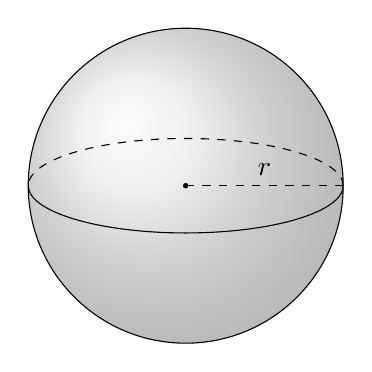
\begin{tikzpicture}
INSERT FIGURE OF FALLING APPLE AS AN EXAMPLE
\shade[ball color = gray!40, opacity = 0.4] (0,0) circle (2cm);
 \draw (0,0) circle (2cm);
  \draw (-2,0) arc (180:360:2 and 0.6);
  \draw[dashed] (2,0) arc (0:180:2 and 0.6);
  \fill[fill=black] (0,0) circle (1pt);
  \draw[dashed] (0,0 ) -- node[above]{$r$} (2,0);
\end{tikzpicture}
\end{center}
\begin{center}
\textit{The apple experiences the earth's gravitational pull without them directly touching.}
\end{center}
\noindent Such forces are often times described in science using \textbf{fields}. Say object $S$ (for source) exerts a force on object $T$ (for test) without directly touching it. This force is described in $2$ steps:
\begin{itemize}
\item Object $S$ creates a field all around it. It is the \textbf{source} of the field. This field is said to be present even if no test particle is present to experience its effect.
\item Object $T$ \textbf{experiences} the effect of the field (or conventionally, it "tests" the force). 
\end{itemize}
\noindent This $2$-step approach to forces allows us to distinguish the effects due to the source from those due to the test object. We introduce these concepts here because electric and magnetic forces are such forces at a distance. Also, their description using fields will be very handy when going into more advanced topics such as electromagnetic waves and radiation.\\

\subsection{Charges and forces}

\noindent Objects have a property known as mass. We all know it because many of us, including yours truly, struggle to keep ours in check. But the question of what this mass really is turns out to be more difficult than you may think. It is actually complicated enough to have merited a nobel prize in physics (2013) for François Englert and Peter Higgs for coming up with a mechanism by which elementary particles get their mass. For most of us mere mortals, we simply have to accept that mass is one of the properties that objects just have, without questioning what this mass really is\footnote{I do not mean to discuss mass in this part of the text, but I introduce wrote this couple of lines about it in the hope of thwarting questions that I am pretty sure will follow concerning the nature of charge.}.\\

\noindent Another such property that objects have is called \textbf{electric charge} (usually we just call it charge and omit the word electric). I cannot tell you what this charge is in the same way I cannot tell you what mass is. We just have to accept that things in reality have a property we call charge. Just as the unit used for mass in science is usually kilogram, so the unit of charge is \textbf{Coulomb}. The basic question being addressed in electromagnetism is "what is the force exerted by an electric charge on another?". The answer as we will see below is that charges exert both electric and magnetic forces on each other.

\subsection{Electricity}

\noindent It has been known since the $17^{th}$ century that there are $2$ kinds of electric charge. Benjamin Franklin, a scientist, political thinker and one of the founding fathers of the USA, called one of the $2$ kinds \textbf{positive} and the other \textbf{negative}, which is how they are still labeled today. Do keep in mind that this is just a name and they may as well have been called green and blue or spoons and forks. The name we give them should not, and does not alter their behavior in any way.\\

\noindent Any $2$ charges always exert a force on each other. If they are of the same kind (both positive or both negative) they repel each other. Otherwise they attract each other. This force is known as the \textbf{electrostatic} or the \textbf{Coulomb force}. It is this force that makes your hairs rise when when taking off a woolen sweater on a cold, dry winter's day.

\noindent To describe this force we start with a single charged particle\footnote{An object with a mass of for instance $5$ kilograms will often be described as "a mass of 5 kilograms". A charged particle with a charge of $2$ Coulombs will often be described as "a charge of $2$ Coulombs".} with a charge we will call $Q_1$ (which for the sake of the discussion below we choose positive). We say that this generates an electric field $\vec{E}$ all around it.
\begin{center}
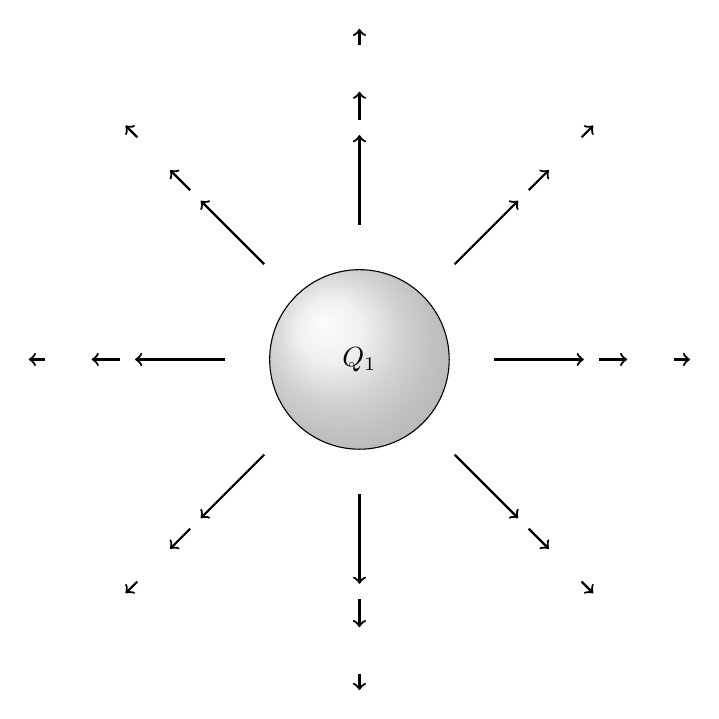
\begin{tikzpicture}[scale=3.8]
\shade[ball color = gray!40, opacity = 0.4] (0,0) circle (3mm);
 \draw (0,0) circle (3mm);
\node at (0,0) {$Q_1$};
\foreach \a in {0,45, 90, 135, 180, 225, 270, 315} {
 \draw[->, thick] (\a:4.5mm) -- (\a:7.5mm);
\draw[->, thick] (\a:8mm) -- (\a:8.949219mm);
\draw[->, thick] (\a:10.5mm) -- (\a:11.05102mm);
}
	\end{tikzpicture}
\end{center}
\noindent What is the meaning of this electric field $\vec{E}$, sketched as the set of arrows above? It represents the force a test charge of $1$ Coulomb would feel, if we were to put it at that point. The direction of the arrow is the direction of the force, and the strength of the force is represented by the length of each arrow. The electric field of a charge (of $1$ Coulomb) points away from the charge, and weakens as we move away from it.

\subsection{Magnetism}
\label{Discuss_Magnet}

\noindent Any $2$ charges exert an electrostatic force on each other. But the actual force between charges is in general more complicated than that. Whenever charges are in motion, they exert, on top of the electrostatic force, an additional force known as the \textbf{magnetic} force or the \textbf{Lorentz force}. This force can also be described using the same $2$-step approach of fields: a source creates the magnetic field all around it and a test particle experiences the forces when it is in the field.\\

\noindent The source of electric field are charges. But when a charge is in motion, it also creates an additional magnetic field $\vec{B}$. As electric currents are nothing but a collection of charges moving, electric currents are sources of magnetic fields.
\begin{figure}[h!]
\centering
  \includegraphics[width=8cm]{Figures/magnetic_field_of_current.jpg}
  \caption{A straight wire in which a current flows generates circular magnetic fields around itself}
\end{figure}
\noindent To see the effect of this magnetic field, a test particle is placed in it. Any charge placed in an electric field experiences the electrostatic force. But only moving charges experiences the magnetic force. Whenever a charge is standing still in a magnetic field, it experiences no magnetic force.\\ 

\subsubsection{Magnets on fridge doors}

\noindent We claim that only moving charges produce magnetic fields, and only moving test charges experience the magnetic force. But if this is so, why are magnets attached to fridges? There do not seem to be any moving charges there.\\

\noindent Good question! I am glad you asked. There are indeed moving charges both in the fridge and in the magnets themselves. They are made of atoms in which protons and electrons, both of which have electrical charges, are moving around. So there is absolutely no lack of moving charges.\\

\noindent But everything is made of atoms in which protons and electrons are moving about. So why are not all objects magnetic?\\

\noindent Another excellent question! All objects indeed have moving charges in them. But the direction of motion of the charges in most objects is random. So each atom in the object indeed behaves like a tiny magnet, but each magnet points in a different direction. And the total effect of all these randomly pointing magnets is that they cancel each other out so that no net magnetic effect remains. In some materials, there is a (quantum) phenomenon known as exchange interaction, which makes it more probable for neighboring atoms to align their magnets.  If this exchange interaction is strong enough (as it is for instance in iron), it can cause a very large number of atoms to align their magnets and cause a strong net magnetic effect. This magnetic phenomenon is known as \textbf{ferromagnetism}. It is this effect that makes magnets hang on the door of our fridges.\\
DISCUSSION OF PARAMAGNETISM AND DIAMAGNETISM

\subsection{Electromagnetism}

\noindent So charges always generate electric fields. When in motion they also give rise to magnetic fields. But it does not stop there. It turns out that when electric fields change with time, they themselves give rise to additional magnetic fields. And when magnetic fields change they generate electric fields.\\

\noindent The electric field caused by a changing magnetic field is known as the \textbf{induced} electric field. A very large part of the electricity we use at home is generated by this principle known as \textbf{Faraday's law of induction}. A wheel is turned around by some external force (falling water, wind, steam$\cdots$). The wheel is attached to a magnet which turns with it. As the magnet turns, its magnetic field changes and induces an electric field which causes an electric current to flow. When the magnet stops turning, the electric flow stops too.\\

\noindent Below is a table summarizing our discussion of electromagnetism.
\begin{center}
\begin{tabular}{|c|c|c|}
\hline 
Source & Fields & Test particle\\
\hline
\hline
\begin{tabular}{c} Electric charge \\ Changing magnetic field \end{tabular} & $\vec{E}$ & Electric charge \\
\hline
\begin{tabular}{c} Moving electric charge \\ Changing electric field \end{tabular} & $\vec{B}$ & Moving electric charge \\
\hline
\end{tabular}
\end{center}
\noindent The answer to the question "what is the force between $2$ " electric charges involves both electric and magnetic fields. Moreover, changing electric fields generate magnetic fields and vice versa. There is indeed a very close connection between the fields. For now they are different though closely related phenomena. We will see in section \ref{RelativeElectrMagn} when discussing relativity that their relation is even closer, that they really are different instances of the same phenomenon.

\subsection{Maxwell's equations and electromagnetic waves}

\noindent In 1870 James Clerk Maxwell published a set of 4 equations that summarized all the known electromagnetic phenomena of this time. Written in today's common physics jargon they are:
\begin{center}
\begin{tabular}{|cll||cll|}
\hline  
& & & & & \\
(I) & $ \vec{\nabla} \cdot \vec{E}$ & $= \frac{\rho }{\epsilon_0} $ & (II) & $\vec{\nabla} \cdot \vec{B} $ & $= 0 $ \\ & & & & & \\
(III) & $ \vec{\nabla} \times \vec{E} $ & $ = -\frac{\partial \vec{B}}{\partial t} $ & (IV) & $ \vec{\nabla} \times \vec{B} $ & $ = \mu_0 \vec{J} + \mu_0 \epsilon_0 \frac{\partial \vec{E}}{\partial t} $ \\ & & & & & \\
\hline
\end{tabular}
\end{center}
\noindent These describe quantitatively the physics I sketched in words above. The exact mathematical meaning of each of the symbols is not for now. But except for the second equation we have already covered all they say.
\begin{enumerate}[I]
\item The electric field $\vec{E}$ is generated by the presence of charges denoted by $\rho$.
\item Magnets have $2$ sides which are conventionally called their north and south pole. This equation says that these poles always come in pairs, that it is impossible to have one without the other. If we take a magnet with a north and a south pole and break it, we are not left with $1$ north and $1$ south pole, but with rather with $2$ magnets, each with its own north and south pole.
\begin{figure}[h!]
\centering
  \includegraphics[width=8cm]{Figures/breaking_bar_magnet.jpg}
  \caption{No matter how it is broken up, a magnet always has both a north and a south pole}
\end{figure}
\item Changing magnetic fields represented by the cryptic looking symbols $\frac{\partial \vec{B}}{\partial t}$ give rise to electric fields.
\item Electric currents represented by $\vec{J}$ and chaning electric fields represented by $\frac{\partial \vec{E}}{\partial t}$ generate magnetic fields.
\end{enumerate}
\noindent Playing around with the equations is not only fun, but it can actually lead to new insights. Some juggling with the equations shows that the electric field $\vec{E}$ and the magnetic field $\vec{B}$ both wave about.
\begin{center}
  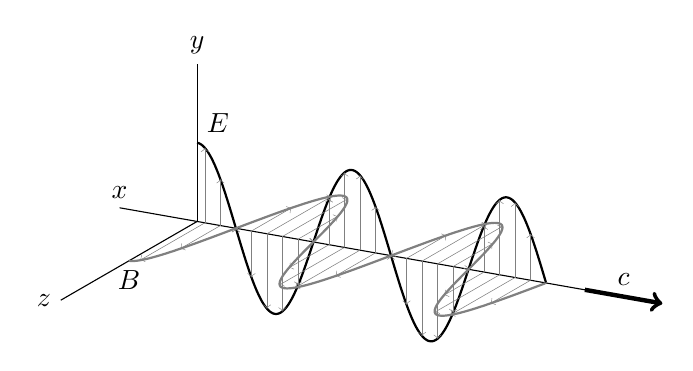
\begin{tikzpicture}[x={(-10:1cm)},y={(90:1cm)},z={(210:1cm)}]
     Axes
    \draw (-1,0,0) node[above] {$x$} -- (5,0,0);
    \draw (0,0,0) -- (0,2,0) node[above] {$y$};
    \draw (0,0,0) -- (0,0,2) node[left] {$z$};
     Propagation
    \draw[->,ultra thick] (5,0,0) -- node[above] {$c$} (6,0,0);
     Waves
    \draw[thick] plot[domain=0:4.5,samples=200] (\x,{cos(deg(pi*\x))},0);
    \draw[gray,thick] plot[domain=0:4.5,samples=200] (\x,0,{cos(deg(pi*\x))});
     Arrows
    \foreach \x in {0.1,0.3,...,4.4} {
      \draw[->,help lines] (\x,0,0) -- (\x,{cos(deg(pi*\x))},0);
      \draw[->,help lines] (\x,0,0) -- (\x,0,{cos(deg(pi*\x))});
    }
     Labels
    \node[above right] at (0,1,0) {$\bm{E}$};
    \node[below] at (0,0,1) {$\bm{B}$};
  \end{tikzpicture}
\end{center}
\noindent The equations predict the existence of wave-like behavior in electric and magnetic fields. And these waves propagate according these same equations at a speed of $1/\sqrt{\mu_0 \epsilon_0}$ which is equal to $299 792 458$ kilometers per second. By playing around with the Maxwell equations it is possible to find a wave in these hypothetical concepts of electric and magnetic fields, which apparently move about at a speed which coincidently brings the speed of light to mind.

\subsection{Relativity: the absoluteness of our shared reality}
\label{RelativeElectrMagn}
\noindent We all live in the same world, in the same reality. There is no obvious reason for the laws of nature observed by one person to be any different from those observed by another. That is the essence of the theory of relativity. A more accurate name would probably be the theory of absoluteness: the laws of physics are the same no matter who looks at the world.\\

 And there is no reason to expect that the laws of nature should depend on who is looking at the world.

In everyday life it may seem that the statement "` if two things happen at the same time from my point of view then they happen at the same time from everyone's point of view"' is correct. Imagine I look at two car accidents occurring at exactly the same instant of time a couple of meters away from each other. If you saw the accidents as well, it seems reasonable to expect you to agree that accidents were indeed simultaneous. But reasonable or not, it is not generally true. You are certain you saw one of the accidents happen a couple of seconds, maybe even minutes, before the other one. A third witness may say the exact opposite, that the accident you claim happened first was actually the second one. Is one or several of us mistaken? Maybe. But it turns out that it is possible for all of to be correct too, as weird as it may sound. The idea that things happen at the same time, or that the order of which event happened first is a given is not always true. And what is even more interesting and surprising is that the fact that it is untrue can be derived by assuming that the speed of light is finite. It is absolutely not trivial to see how an assumption about the speed of light can influence the flow of time or the order of events, but its true nonetheless. Math allows us to think in a formal and logical way about the consequences of assumptions even when they do not seem intuitive or obvious. 

\subsection{Electromagnetism and the animal world}

Platypus:
The mystery of how platypuses catch their prey in murky water at night, with their eyes, ears, and nostrils closed, puzzled scientists for years. Then researchers discovered that, unlike any other land mammal, platypuses use the electrical impulses emitted by their prey to home in on a meal.
A platypus’ bill is covered in nearly 40,000 electricity sensors—or electroreceptors—arranged in a series of stripes, which helps them localize prey. All animals produce electric fields due to the activity of their nerves and muscles. So when the platypus digs in the bottom of streams with its bill, its electroreceptors detect these tiny currents, allowing it to tell living prey from inanimate objects.\\

Oriental hornet
The Oriental hornet is a truly solar-powered animal: Its exoskeleton is capable of transforming solar energy into electricity.
Unlike most hornets that avoid activity during the hottest part of the day, Oriental hornets are out in force when the sun is most intense. The brown-and-yellow-striped insects do this to harvest the sun’s energy.
The brown stripes trap sunlight, while the yellow stripes convert the sunlight into electricity.
What do Oriental hornets do with this homegrown electricity? Experts aren’t sure, but some research finds the electricity could help the insects create enzymes that aid in their metabolism. It could also help keep the hornets comfortable even at high temperatures; they can stay cool by converting heat energy into electricity, which they can then store and convert back into heat when it cools down.
Alternatively, the electricity might give their wing muscles an energy boost. Shining ultraviolet light on anesthetized hornets made them wake up faster and immediately fly away, as if it recharged their batteries.\\

Bees
A flower's bright petals and fragrance aren't the only things that attract bees. Flowers often experience a change in electric charge after they've been visited, so by sensing electric fields, bees can decide whether a flower is worth investigating (or if someone got there before them).

\subsection{Electromagnetism: not just for animals}

\noindent Below are a number of other ways electromagnetism is used outside of daily life.
\begin{itemize}
\item Brain mapping using electric currents and their induced magnetic fields
\item Study of earth's core using its magnetic field
\end{itemize}

%\section{The sound of music}
%
%\noindent basics of sound
%% Dog whistles: sounds, their meaning, the limitations of experiencing them, sonar and the bat
%
%\section{Light illuminated}
%
%\noindent Light
%% Light and visibility and what animals experience: why bees can only see some colors. And that birds see infrared and are coloured in those frequencies. The stripes of the zebra. how do animals "see" if they live very deep under water
%
%%\section{Find order in all the chaos}
%%
%%\noindent Predictability, chaos and determinism
%% Predator-Prey models: Lotka-Voltera
%% Lyapunov exponents, Lorenz attractors and weather prediction
%
%\section{The solace of quantum}
%
%\noindent Now we get to the real stuff. Allow me introduce you to the world of the quantum, where things are and are not, statements may have a certain meaning, or maybe another meaning, no meaning at all, or all meanings simultaneously...\\
%\noindent Or something like that...\\
%\noindent Welcome to the wondrous world of quantum physics.\\
%
%\noindent Before I start discussing a topic as sensational as this one, let me caveat some of what is to come with a couple of preemptive remarks:
%\begin{itemize}
%\item Quantum physics and its extension to relativistic systems known as quantum field theory are among the most accurate and well-tested ideas humans have ever had. There are no known phenomena that are in contradiction with the predictions of the quantum theory.
%\item Despite it sounding esoteric and woolly, quantum physics is a very precise scientific theory that makes exact statements about reality, some of which seem weird when one is not used to the quantum world. Consequently, the theory has been misinterpreted and misused by some, claiming it says things much vaguer and more extraordinary than it actually does. As a general word of warning, beware of statements whose merit only lies in their sounding equally mind-boggling and mysterious to the untrained ear. The arguments sound a bit like this:
%\begin{enumerate}[*]
%\item A is weird, esoteric and as far as we can tell, describes reality very accurately (A being my very metaphorical representation of all that is quantum).
%\item B is equally weird and esoteric as A (B being any esoteric quack statement).
%\item Therefore B is equally true as A.
%\end{enumerate}
%\noindent I do not claim that $B$ is necessarily untrue. But the argument as such is not logically correct and if the claimer feels the need to resort to such a falsehood, it should at least make you wary of its truth.
%\item One often hears that classical mechanics as developed by Newton, Leibniz, Lagrange and others is wrong and has been replaced by quantum physics. It is important not to read too much into this. Classical mechanics describes the behavior of a football, a sailing boat and a violin quite accurately. In fact, the description is so accurate that we never encounter deviations from the predictions made by classical physics for such systems in daily life. But there are other systems such as atoms, electrons and light where the predictions of classical physics do contradict what is observed in reality when looked at more closely, on scales unavailable to us in our daily life. For such systems a quantum description is needed.\\
%
%\noindent Normal everyday objects such as watches and chocolate cakes obey the laws of classical physics while their constituents - atoms, protons, electrons and others - obey those of quantum physics. We therefore demand that when describing an everyday object like a table starting from the quantum description of its constituents, it gives rise to the laws of classical physics. In other words classical physics needs to be a result of applying quantum physics to a very large number of atoms together. In this sense classical physics should be thought of as a special case of the more general quantum theory.
%\end{itemize}
%\noindent Enough caveating! In the following sections I will describe a number of experiments whose observed results cannot be accounted for by classical physics. Remember that if these observations seem weird to you, it is because they are. Once again, welcome to the world of quantum!
%
%\subsection{So many slits, so few balls}
%
%\noindent Physical phenomena can be divided into two main categories: particles and waves. At least, that is what was believed until the early $20^{th}$ century. Today this dichotomy is understood to be false. In order to understand what was believed and in what sense it is wrong we consider each of its two parts separately.
%
%\subsubsection{If I were a tennis ball}
%
%\noindent On the left is a machine that shoots out a tennis ball every $10$ seconds towards a wall. It can do so in any direction (within the thin dotted lines) by rotating around its own axis (the figure below shows the set-up as seen from above). Behind the wall is a screen used for counting the number and location of balls hitting it. In this case none of the tennis balls will reach the screen as they will all be stopped by the wall. The trajectories of $3$ tennis balls are shown. All are blocked by the wall, where the points of impact are marked by a \huge{$\times$}\normalsize.
%\begin{center}
%\begin{tikzpicture}
%\draw[ultra thick] (0,-3)--(0,3)node[above]{Wall};
%\draw[thick] (2,-3)--(2,3)node[above]{Screen};
%\filldraw (-4.2,-0.2) rectangle (-3.8,0.2);
%\node at (-4,3)[above]{Ball thrower};
%\draw[very thin,gray,dotted] (-4,0)--(0,2.8);
%\draw[very thin,gray,dotted] (-4,0)--(0,-2.8);
%\draw[black!50!gray,dashed] (-4,0) -- (0,0.2);
%\node[ultra thick,black] at (0,0.2){\huge $\times$};
%\draw[black!50!gray,dashed] (-4,0) -- (0,2);
%\node[ultra thick,black] at (0,2){\huge $\times$};
%\draw[black!50!gray,dashed] (-4,0) -- (0,-1.5);
%\node[ultra thick,black] at (0,-1.5){\huge $\times$};
%\end{tikzpicture}
%\end{center}
%\noindent We now make a small hole somewhere in the wall, large enough so that a ball can get through it, but not much larger than that. Most thrown tennis balls will be blocked by the wall. But those that happen to be thrown in the direction of the hole will get through and hit the screen. We mark the point of impact by \tikz{\filldraw (0,0) circle [radius=1.5pt];}. By way of example, I drew $3$ of the balls that pass through the hole. The screen has electronic sensors which allow us to determine where and how many balls hit it. At the end of the experiment the machine outputs a graph which represents the hits each part of the screen recorded, shown on the right. 
%\begin{center}
%\begin{tikzpicture}
%\draw[ultra thick] (0,-3)--(0,-1.75);
%\draw[ultra thick] (0,-1.25)--(0,3)node[above]{Wall};
%\draw[thick] (2,-3)--(2,3)node[above]{Screen};
%\filldraw (-4.2,-0.2) rectangle (-3.8,0.2);
%\node at (-4,3)[above]{Ball thrower};
%\draw[very thin,gray,dotted] (-4,0)--(0,2.8);
%\draw[very thin,gray,dotted] (-4,0)--(0,-2.8);
%\draw[black!50!gray,dashed] (-4,0) -- (0,0.2);
%\node[ultra thick,black] at (0,0.2){\huge $\times$};
%\draw[black!50!gray,dashed] (-4,0) -- (0,1.5);
%\node[ultra thick,black] at (0,1.5){\huge $\times$};
%\draw[black!50!gray,dashed] (-4,0) -- (2,-2.25);
%\filldraw (2,-2.25) circle[radius=1.5pt];
%\draw[black!50!gray,dashed] (-4,0) -- (2,-2.46);
%\filldraw (2,-2.46) circle[radius=1.5pt];
%\draw[black!50!gray,dashed] (-4,0) -- (2,-2.1);
%\filldraw (2,-2.1) circle[radius=1.5pt];
%\end{tikzpicture}
%\begin{tikzpicture}
%\end{tikzpicture}
%\begin{tikzpicture}[rotate=90]
	%\draw[smooth, domain = -3:-1.5, ultra thick, black] plot function{2*exp(-225*(x+2.25)*(x+2.25))};
	%\draw[smooth, domain = -1.5:3, ultra thick, black] plot function{0};
	%\node[above] at (3,0){Output};
%\end{tikzpicture}
%\end{center}
%\noindent The output indeed shows a peak at the point where the tennis ball hit the screen, and nothing elsewhere, as expected. We now make a second hole in the wall, and let the experiment run for a couple of hours. The set-up and the corresponding output is shown below.
%\begin{center}
%\begin{tikzpicture}
%\draw[ultra thick] (0,-3)--(0,-1.75);
%\draw[ultra thick] (0,-1.25)--(0,1.25);
%\draw[ultra thick] (0,1.75)--(0,3)node[above]{Wall};
%\draw[thick] (2,-3)--(2,3)node[above]{Screen};
%\filldraw (-4.2,-0.2) rectangle (-3.8,0.2);
%\node at (-4,3)[above]{Ball thrower};
%\draw[very thin,gray,dotted] (-4,0)--(0,2.8);
%\draw[very thin,gray,dotted] (-4,0)--(0,-2.8);
%\draw[black!50!gray,dashed] (-4,0) -- (0,0.2);
%\node[ultra thick,black] at (0,0.2){\huge $\times$};
%\draw[black!50!gray,dashed] (-4,0) -- (2,2.25);
%%\node[ultra thick,black] at (0,1.5){\huge $\times$};
%\draw[black!50!gray,dashed] (-4,0) -- (2,-2.25);
%\filldraw (2,-2.25) circle[radius=1.5pt];
%\filldraw (2,2.25) circle[radius=1.5pt];
%\end{tikzpicture}
%\begin{tikzpicture}
%\end{tikzpicture}
%\begin{tikzpicture}[rotate=90]
	%\draw[smooth, domain = -3:-1.5, ultra thick, black] plot function{2*exp(-225*(x+2.25)*(x+2.25))};
	%\draw[smooth, domain = -1.5:1.5, ultra thick, black] plot function{0};
	%\draw[smooth, domain = 1.5:3, ultra thick, black] plot function{2*exp(-225*(x-2.25)*(x-2.25))};
	%\node[above] at (3,0){Output};
%\end{tikzpicture}
%\end{center}
%\noindent The result is not really surprising. We indeed expect to see a peak behind each hole and no recorded hits elsewhere\footnote{Though improbable, it is possible for the tennis balls to not simply pass through the hole but hit one of its sides and be scattered in a different direction. Therefore, it is to be expected that a small number of hits will be recorded away from the two shown peaks on the output. Nevertheless, it remains true that two main peaks will appear as shown in the figure.}. 
%
%\subsubsection{If I were a water wave}
%
%\noindent Waves exhibit quite a different behavior. You have undoubtedly already noticed when throwing a rock in a pond the circular waves appearing on its surface, moving away from the point of impact.
%\begin{center}
%\begin{tikzpicture}
%\filldraw (0,0) circle (0.8mm);
%\draw[->, dashed, very thick] (0.1 cm,0.1 cm) -- (1.7 cm,1.7 cm);
%\draw[->, dashed, very thick] (- 0.1 cm, 0.1 cm) -- (-1.7 cm,1.7 cm);
%\draw[->, dashed, very thick] (0 cm,- 0.1 cm) -- (0 cm,-2.4 cm);
%\foreach \x in {0.5,1,...,2.5}
%\draw (0,0) circle [radius=\x cm];
%\foreach \x in {0.25,0.75,...,2.25}
%\draw[gray, dotted] (0,0) circle [radius=\x cm];
%\end{tikzpicture}
%\end{center}
%\noindent The water wave consists of alternating peaks and throughs \\
%
%\noindent ADD INTRODUCTION ABOUT PLANE WAVES, DIFFRACTION AND HUYGHENS PRINCIPLE\\
 %
%\noindent When the waves arrives at the wall, it will be split up and two spherical waves will leave the slits.
%\begin{center}
%\begin{tikzpicture}
%\draw[ultra thick] (0,-3)--(0,-1.75);
%\draw[ultra thick] (0,-1.25)--(0,1.25);
%\draw[ultra thick] (0,1.75)--(0,3)node[above]{Wall};
%\draw[thick] (2,-3)--(2,3)node[above]{Screen};
%\filldraw (-4.2,-0.2) rectangle (-3.8,0.2);
%\node at (-4,3)[above]{Source of waves};
%\end{tikzpicture}
%\begin{tikzpicture}
%\end{tikzpicture}
%\begin{tikzpicture}[rotate=90]
	%\draw[smooth, domain = -3:3, ultra thick, black, samples=1500] plot function{cos(3.14*4*sin(x))*cos(3.14*4*sin(x))*(sin(3.14*2*sin(x))/(3.14*2*sin(x)))*(sin(3.14*2*sin(x))/(3.14*2*sin(x)))};
	%\node[above] at (3,0){Output};
%\end{tikzpicture}
%\end{center}
%
%\subsubsection{I am that I am}
%
%\noindent Testing whether something is a particle or a wave should not be too hard. Is light a wave? If so, an interference pattern should be observed when shining a light towards a wall with $2$ thin slits\footnote{Add a footnote about the size of the slit relating to the "size" of the particles}. Is an electron a particle? If so, a pattern of $2$ peaks behind the slits should be found as with tennis balls.\\
%
%\noindent The classification of things into waves or particles is a human-made one. Nature feels no obligation (moral or otherwise) to obey. It just does what it does. And if reality does not comply, it is up to us to change our description of it.\\
%
%\noindent What is actually observed when doing this experiment with electrons? Here is a list of observed facts:
%\begin{enumerate}[i]
%\item When electrons are sent one every $10$ seconds, the screen behind the slits records a hit every $10$ seconds. Each hit is localized, meaning that the screen records the hit at a specific location (as would be the case if electrons were particles).
%\item Though each electron causes a localized hit on the screen, after a very large number of hits, the distribution on the screen of the hits is an interference pattern (as would be expected if electrons were waves).
%\item DESCRIBE EFFECT OF LOCATING SLIT OF ENTRANCE
%\end{enumerate}
%\noindent Though there are several aspects of this that seem surprising, I want to emphasize that the fact of electrons behavior neither as waves nor particles is as such not magical. We tried classifying them into groups that are simply not a correct way of describing reality. Things are not one or the other. Nor are they both. Things simply are what they are. And they behave the way real things do. And this real behavior has some common properties to particles and others common to waves. But real things are neither. The thing they are is known as wave-particle.\\
%
%\noindent Doing this experiment with light yields similar results. It turns out light is also particle nor wave. Both electrons and light behave as wave-particles. The experiment has been further done with larger things like molecules. And they also are wave-particles. All the building-blocks of nature (though the word building-block is reminiscent of a particle-like nature) are actually wave-particles. 
%
%\subsection{Tiny magnets flying all over the place}
%
%\noindent We have seen earlier that a moving magnet will be deflected from its straight trajectory when passing through a magnetic field. The question we consider here is whether elementary particles like electrons, protons and neutrons behave as if they were tiny magnets. Are their trajectories deflected by magnetic fields. The short answer is, yes they are. Every elementary particle has a property called its \textbf{magnetic moment} which tells us how "tiny magnet"-like it behaves (or how strongly it interacts with a magnetic field if phrased in a somewhat more sciency lingo). It turns out, for reasons I will not go into here, that the magnetic moment of neutrons\footnote{Electrons and protons have a spin as well. But we know that moving charges are influenced by magnetic fields. The magnetic deflection of their trajectories would therefore be due to $2$ effects: partially from their charge and partially from their spin. As neutrons are electrically neutral the effect of the magnetic field can be studied in isolation. The experiment described above is actually more often executed with electrically neutral silver atoms for practical reasons but the description of the phenomenon above holds true.} depends on a property of theirs known as their \textbf{spin}. 
%
%Actually, both the magnetic moment and the spin are three properties rather than one. Let us call the vertical direction the $z$ direction, and the two horizontal direction the $x$ and $y$ directions. Every particle has three magnetic moments and three spins: one in each of these directions. A magnetic field in the $z$-direction will be 
%
%And this spin is a rather weird property which exhibits some highly quantum behavior. The spin is actually not one but three quantities: one for every perpendicular direction. If we call the vertical direction the $z$ direction, it is the spin in $z$-direction that will determine by how much the particle will be deflected in vertical direction. There is thus a spin in every one of the three dimension, usually denoted by $S_x$, $S_y$ and $S_z$. Which direction gets each of these labels is completely arbitrary and has no importance at all. 
%
%Do not try too hard to "understand" what this spin is. It suffices for now to say that it is NOT the speed of rotation of these particles around their own axis. 
%
%Actually, each of these particles has three different and in some sense independent spin
%
%\subsection{The Bells of inequality: how real is reality?}
%
%\noindent You think spins and slits are weird? Wait until you hear this...\\
%
%\noindent In the classical world, objects have properties independently of whether they are directly visible to the world or not. In stark contrast, the quantum theory claims there are situations in which some properties of a system are not determined until they are actually tested.\\
%
%\noindent To make this more concrete and accessible, I will describe below a system where this distinction between the classical and the quantum predictions is blatant. Let us think of a toy cube. Just a solid toy cube with $6$ sides/faces. Actually, think of a bag with many such toy cubes. Each cube has $2$ sides painted either red or blue. On $2$ of its other sides can be found either the symbol $V$ or the symbol $X$. And on the remaining $2$ sides is either a happy smiley or a sad smiley\footnote{By happy smiley I mean \Smiley and by sad smiley \Sadey}. All the cubes in the bag have the property that opposing faces are identical. So that if one of the faces of the cube has the symbol $X$ on it, the opposite face must also have an $X$. Here are different views of one such cube.
%\begin{center}
%\begin{tikzpicture}[on grid, scale=0.6]
  %\shade[yslant=-0.5,right color=white!50!gray, left color=white!10!gray] (0,0) rectangle +(3,3); % Left face
  %\shade[yslant=0.5,right color=white!10!gray,left color=white!50!gray] (3,-3) rectangle +(3,3); % Right face
  %\shade[yslant=0.5,xslant=-1,bottom color=blue!20!white,
    %top color=blue!60!white] (6,3) rectangle +(-3,-3); % Top face
	%\draw[yslant=-0.5] (0,0) rectangle (3,3);
	%\draw[yslant=0.5] (3,-3) rectangle (6,0);
	%\draw[yslant=0.5,xslant=-1] (3,0) rectangle +(3,3);
	%\node[yslant=-0.5] at (1.5,0.75) {\Huge $\bm{V}$};
	%\node[yslant=0.5] at (4.5,0.75) {\Huge \Smiley};
%\end{tikzpicture}
%\begin{tikzpicture}[on grid, scale=0.6]
  %\shade[yslant=-0.5,right color=white!50!gray, left color=white!10!gray] (0,0) rectangle +(3,3); % Left face
	%\shade[yslant=0.5,right color=blue!60!white,left color=blue!20!white] (3,-3) rectangle +(3,3); % Right face
  %\shade[yslant=0.5,xslant=-1,bottom color=white!50!gray,
    %top color=white!10!gray] (6,3) rectangle +(-3,-3); % Top face
	%\draw[yslant=-0.5] (0,0) rectangle (3,3);
	%\draw[yslant=0.5] (3,-3) rectangle (6,0);
	%\draw[yslant=0.5,xslant=-1] (3,0) rectangle +(3,3);
	%\node[yslant=-0.5,rotate = -90] at (1.5,0.75) {\Huge $\bm{V}$};
	%\node[yslant=0.5, xslant=-1, rotate=180] at (3,3) {\Huge \Smiley};
%\end{tikzpicture}
%\begin{tikzpicture}[on grid, scale=0.6]
	%\shade[yslant=-0.5,right color=blue!20!white, left color=blue!60!white] (0,0) rectangle +(3,3); % Left face
	%\shade[yslant=0.5,right color=white!50!gray,left color=white!10!gray] (3,-3) rectangle +(3,3); % Right face
  %\shade[yslant=0.5,xslant=-1,bottom color=white!50!gray,
    %top color=white!10!gray] (6,3) rectangle +(-3,-3); % Top face
	%\draw[yslant=-0.5] (0,0) rectangle (3,3);
	%\draw[yslant=0.5] (3,-3) rectangle (6,0);
	%\draw[yslant=0.5,xslant=-1] (3,0) rectangle +(3,3);
	%\node[yslant=0.5,rotate = 90] at (4.5,0.75) {\Huge $\bm{V}$};
	%\node[yslant=0.5, xslant=-1, rotate=90] at (3,3) {\Huge \Smiley};
%\end{tikzpicture}
%\end{center}
%\noindent This cube has $2$ blue faces, $2$ faces with a happy smiley and $2$ faces with a $V$ symbol. A second cube may look like this:
%\begin{center}
%\begin{tikzpicture}[on grid, scale=0.6]
  %\shade[yslant=-0.5,right color=white!50!gray, left color=white!10!gray] (0,0) rectangle +(3,3); % Left face
  %\shade[yslant=0.5,right color=white!10!gray,left color=white!50!gray] (3,-3) rectangle +(3,3); % Right face
  %\shade[yslant=0.5,xslant=-1,bottom color=red!20!white,
    %top color=red!60!white] (6,3) rectangle +(-3,-3); % Top face
	%\draw[yslant=-0.5] (0,0) rectangle (3,3);
	%\draw[yslant=0.5] (3,-3) rectangle (6,0);
	%\draw[yslant=0.5,xslant=-1] (3,0) rectangle +(3,3);
	%\node[yslant=-0.5] at (1.5,0.75) {\Huge $\bm{X}$};
	%\node[yslant=0.5] at (4.5,0.75) {\Huge \Smiley};
%\end{tikzpicture}
%\end{center}
%\noindent This second cube has $2$ red faces, $2$ faces with the symbol $X$ on them and $2$ faces with a happy smiley.\\
%
%\noindent To get to the heart of the weirdness of the quantum world we need to add a small complication. Imagine that each of these cubes is fitted with a tight cloth covering it. The cloth has only $1$ small hole in it, allowing us to see only $1$ of its faces at a time. It is nevertheless possible to wiggle and turn the cube within this cloth so as to see each of its faces in turn.
%\begin{center}
%\begin{tikzpicture}[on grid, scale=0.6]
	%\filldraw[yslant=-0.5, gray] (0,0) rectangle (3,3);
	%\draw[yslant=-0.5, color=white!30!gray] (0,0) rectangle +(3,3);
	%\filldraw[yslant=0.5,xslant=-1, gray] (3,0) rectangle +(3,3);
	%\draw[yslant=0.5,xslant=-1, color= white!30!gray] (3,0) rectangle +(3,3);
	%\filldraw[yslant=0.5, gray] (3,-3) rectangle +(3,3);
	%\draw[yslant=0.5, color=white!30!gray] (3,-3) rectangle +(3,3);	
	%\shade[yslant=0.5,right color=white!10!gray,left color=white!50!gray] (4.5,-1.5) ellipse [x radius= 25pt, y radius = 35pt]; % Right face
	%\node[yslant=0.5] at (4.5,0.75) {\Huge \Sadey};
%\end{tikzpicture}
%\begin{tikzpicture}[on grid, scale=0.6]
	%\filldraw[yslant=-0.5, gray] (0,0) rectangle (3,3);
	%\draw[yslant=-0.5, color=white!30!gray] (0,0) rectangle +(3,3);
	%\filldraw[yslant=0.5,xslant=-1, gray] (3,0) rectangle +(3,3);
	%\draw[yslant=0.5,xslant=-1, color= white!30!gray] (3,0) rectangle +(3,3);
	%\filldraw[yslant=0.5, gray] (3,-3) rectangle +(3,3);
	%\draw[yslant=0.5, color=white!30!gray] (3,-3) rectangle +(3,3);	
	%\shade[yslant=0.5,right color=blue!20!white,left color=blue!60!white] (4.5,-1.5) ellipse [x radius= 25pt, y radius = 35pt]; % Right face
%\end{tikzpicture}
%\end{center}
%\noindent This cube has a sad smiley on one of its faces. We know for certain that the face opposite it also has a sad smiley. By moving the cloth around we find that another side is blue. And again we know that the face opposite it is blue too. As we have not seen the other faces we do not know whether they contain an $X$ or a $V$.\\
%
%\noindent The bag is filled with many such cubes. You put your hand into the bag pick one cube out at random, which you put on the table in front of you. You can only see $1$ of its faces.
%\begin{center}
%\begin{tikzpicture}[on grid, scale=0.6]
	%\filldraw[yslant=-0.5, gray] (0,0) rectangle (3,3);
	%\draw[yslant=-0.5, color=white!30!gray] (0,0) rectangle +(3,3);
	%\filldraw[yslant=0.5,xslant=-1, gray] (3,0) rectangle +(3,3);
	%\draw[yslant=0.5,xslant=-1, color= white!30!gray] (3,0) rectangle +(3,3);
	%\filldraw[yslant=0.5, gray] (3,-3) rectangle +(3,3);
	%\draw[yslant=0.5, color=white!30!gray] (3,-3) rectangle +(3,3);	
	%\shade[yslant=0.5,right color=white!10!gray,left color=white!50!gray] (4.5,-1.5) ellipse [x radius= 25pt, y radius = 35pt]; % Right face
	%\node[yslant=0.5] at (4.5,0.75) {\Huge $\bm{X}$};
%\end{tikzpicture}
%\end{center}
%\noindent Even though we do not see the opposite face, we know that no cubes exist where opposite faces differ, so that the invisible opposite face also must contain an $X$. But that is all we can say. We do not know what the other $4$ faces show. One of the most striking differences between classical physics and quantum physics is the following:
%\begin{itemize}
%\item In the \textbf{classical} world, once you pick out a cube, all $6$ of its faces are fixed. Because of the cloth we only know what $2$ of the faces show (the one we see and the one opposite it). The other $4$ sides are unknown to us, but are fixed. They are what they are, and we can discover what they show by moving the hole in the cloth around.
%\item In the \textbf{quantum} world, the $4$ other faces do not have a determined symbol or color until the cloth is turned around and that face is shown. As long as each of the $4$ faces remains hidden, we cannot say that it has a specific color or symbol. Let me emphasize that the statement is stronger than simply saying we do not know what each of the $4$ faces show (which we indeed do not). But rather that nature has not yet "made up her mind", and will only do so when forced to.
%\end{itemize}
%\noindent Notice $2$ important points:
%\begin{enumerate}
%\item The classical and the quantum descriptions agree that the face opposite the visible one is fixed and known. However, they disagree about the $4$ other faces.
%\item The "weird" behavior of a face of a cube not having a determined symbol or color disappears when the face is uncovered. It only does that weirdness when it is covered.
%\end{enumerate}
%\noindent How to determine whether we live in classical world, a quantum world, or another kind of world altogether? The difference between these worlds may seem philosophical rather than scientific. How can there ever be an empirical way to distinguish these world, if every time we look at each face, it indeed shows a specific symbol or color.\\
%
%\noindent Let me introduce John Stewart Bell, a Northern Irish physicist, who in the $1960's$ succeeded in elevating the question from philosophy to physics. He came up with an experiment on how to do it, though he did not actually execute it himself. Below is a simplified version of his suggested experiment.\\
%
%\noindent Take the bag filled with many of these cubes and pick out several cubes consecutively. All we will do is count the number of cubes with each combination of color, symbol and smiley. We will for instance denote the number of cubes we pick out with a blue face, a $V$ and a happy smiley by $N\left( \colorbox{blue!60!white}{\textcolor{blue!60!white}{x}}, V , \Smiley \right)$. The inequality we will test, known as \textbf{Bell's inequality} is
%\begin{equation}
%\label{Bellsinequality}
 %\boxed{N\left( \colorbox{blue!60!white}{\textcolor{blue!60!white}{x}}, X \right) + N\left( V, \Sadey \right) \geq N\left( \colorbox{blue!60!white}{\textcolor{blue!60!white}{x}}, \Sadey \right)}
%\end{equation}
%\noindent When we write $N\left( \colorbox{blue!60!white}{\textcolor{blue!60!white}{x}}, X \right)$ we mean the number of cubes with a blue face and a symbol $X$, independently of whether the smiley is a happy or a sad one. Therefore
%\begin{equation}
%N\left( \colorbox{blue!60!white}{\textcolor{blue!60!white}{x}}, X \right) = N\left( \colorbox{blue!60!white}{\textcolor{blue!60!white}{x}}, X, \Smiley \right) + N\left( \colorbox{blue!60!white}{\textcolor{blue!60!white}{x}}, X, \Sadey \right)
%\label{TwobyTwo}
%\end{equation}
%\noindent Where does Bell's inequality come from? Start from the obviously true inequality
%$$
%N\left( \colorbox{blue!60!white}{\textcolor{blue!60!white}{x}}, X, \Smiley \right) + N\left( \colorbox{red!60!white}{\textcolor{red!60!white}{x}}, V, \Sadey \right) \geq 0
%$$
%\noindent This is true simply because a number of cubes cannot be negative. Now add the same things on both sides of the inequality
%$$
%N\left( \colorbox{blue!60!white}{\textcolor{blue!60!white}{x}}, X, \Smiley \right) + N\left( \colorbox{blue!60!white}{\textcolor{blue!60!white}{x}}, X, \Sadey \right) + N\left( \colorbox{blue!60!white}{\textcolor{blue!60!white}{x}}, V, \Sadey \right) + N\left( \colorbox{red!60!white}{\textcolor{red!60!white}{x}}, V, \Sadey \right) \geq  N\left( \colorbox{blue!60!white}{\textcolor{blue!60!white}{x}}, X, \Sadey \right) 
%+N\left( \colorbox{blue!60!white}{\textcolor{blue!60!white}{x}}, V, \Sadey \right)
%$$
%\noindent And finally, we use equation (\ref{TwobyTwo}) and its analogues to take the terms together two by two. This indeed gives us Bell's inequality.
%$$
%N\left( \colorbox{blue!60!white}{\textcolor{blue!60!white}{x}}, X \right) + N\left( V, \Sadey \right) \geq N\left( \colorbox{blue!60!white}{\textcolor{blue!60!white}{x}}, \Sadey \right)
%$$
%\noindent It follows from the simple and true starting point that a number of cubes cannot be negative. How can it ever be violated when actually counting cubes? And how does it help us at all to determine whether the world is classical or quantum?\\
%
%\noindent There actually is an implicit assumption in the derivation. One that you most probably missed. One that I missed. As did most people until John Bell explicitly pointed it out to us. When we write down something like $N\left( \colorbox{red!60!white}{\textcolor{red!60!white}{x}}, V, \Smiley \right)$, we are actually asserting that it is meaningful to speak of a cube which has a red face, a $V$ and a happy smiley, all at the same time. And in the classical world it indeed makes sense. But in the quantum world the notion of a cube with the colors, symbols and smileys all well-determined simultaneously is simply not meaningful. And so the derivation and its result may well be violated if we are in the quantum world.\\
%
%\noindent In the early $1980'$ a French physicist by the name of Alain Aspect carried out such experiments. The cubes were of course not cubes, but small particles. And the faces of the cubes were some other binary properties\footnote{A property is binary if its result can take on only $1$ of $2$ possible values} of these particles. But the important point is that the Bell inequality is indeed violated. As unbelievable as it may seem, the quantum phenomenon of not having a well-determined property before measuring it turns out to be a correct description of reality. Since the $1980's$ many more experiments have been carried out to test this seemingly crazy result, with results corroborating the quantum predictions. In the quantum world some properties are unknown until they are measured, not because we do not know them, but because nature itself does not yet know.
%
%\subsection{Quantum images: nuclear...? No, I don't want to!}
%
%%%Other things QM is good for:
%%% NMR - MRI
%%% Discretized energy states and spectral lines
%%% Semiconductors and electronics thanks to QM
%%% Heat capacity at low temperatures of crystals
%%% Ferromagnetism
%%% Photo-electric effect
%
%\subsection{The penguin and the pussycat}
%
%\noindent What does an introduction to quantum physics do in a chapter about the physics of animals? You may say to yourself "okay, he can find links between living organisms and surface tension or sound, but surely he won't find such a link with quantum physics". You would more or less be right. Do not misunderstand me. I am by no means claiming that such a link does not exist. As far as we know the world is quantum at its core and everything, including living organisms, obey the laws of quantum physics. But this is only an indirect link. Quantum mechanics gives rise as explained above to classical physics for large systems (like a chair, an eagle or the moon), and animals are among the many such macroscopic systems obeying those laws. But this feels like a cop-out because all we are saying is that classical physics is useful for the animal world, and the quantum laws gives rise to these laws. A quick glance at the recent literature in biology does show some promising direct links between the quantum and the zoological. Unfortunately for me, I am not aware of a biological system where the link with quantum mechanics is sufficiently obvious and straightforward to be of use in an introductory chapter on the subject.\\
%
%\noindent But do not fear!\\
%\noindent I found something that resembles a link between quantum mechanics and the animal world...\\
%
%\subsubsection{Live and let die: a cat's tale}
%
%\noindent Schrodinger's cat
%
%\subsubsection{Penguins decide on magnetic moment}
%
%\noindent When studying advanced quantum mechanics and the phenomeno that occur 
%
%The quote is:\\
%
%\noindent \say{Mary K. [Gaillard], Dimitri [Nanopoulos] and I first got interested in what are now called penguin diagrams while we were studying CP violation in the Standard Model in $1976$... The penguin name came in $1977$, as follows.\\
%
%\noindent In the spring of $1977$, Mike Chanowitz, Mary K and I wrote a paper on GUTs predicting the b quark mass before it was found. When it was found a few weeks later, Mary K, Dimitri, Serge Rudaz and I immediately started working on its phenomenology. That summer, there was a student at CERN, Melissa Franklin who is now an experimentalist at Harvard. One evening, she, I, and Serge went to a pub, and she and I started a game of darts. We made a bet that if I lost I had to put the word penguin into my next paper. She actually left the darts game before the end, and was replaced by Serge, who beat me. Nevertheless, I felt obligated to carry out the conditions of the bet.\\
%
%\noindent For some time, it was not clear to me how to get the word into this b quark paper that we were writing at the time. Then, one evening, after working at CERN, I stopped on my way back to my apartment to visit some friends living in Meyrin where I smoked some illegal substance. Later, when I got back to my apartment and continued working on our paper, I had a sudden flash that the famous diagrams look like penguins. So we put the name into our paper, and the rest, as they say, is history.}
%
%\subsubsection{Concluding remarks}
%
%\noindent Admittedly, the links between animals and quantum are a bit contrived. But quantum physics is so cool that I absolutely could not wait until a next chapter to discuss it. How else could I have discussed such a fascinating topic in a chapter about animals?
%
%
%%Radioactivity and carbon dating
%
%%\section{The reality of doing science}
%%
%%\noindent What science looks in reality and how it compares to what it is thought or said to be.\\
%%
%%\noindent Previously I shortly described the scientific method and its use to asses the validity of statements about reality. But how does this theoretical framework of science compare to what actually happens in the day-to-day life of research scientists?\\
%%
%%\noindent As with any human endeavor, the truth of the matter is that it is more complex and nuanced than may seem from the theoretical concepts. Science is a human activity and is prone to the same glitches and flaws that any other activity may have: popularity of ideas may trump facts, fraudulent results, selective publication of results in order to advance one's career, conservatism concerning accepted ideas and paradigms... 
%
%
%%%%%%%%%%%%%%%%%%%%%%%%%%%%%%%%%%%%%%%%%%%%%%%%%%%%%%%%%%%%%%%%%%
%%\section{Einstein Annus Mirabilis papers}
%%
 %%Topics to cover
 %%Speed of dark. More generally, things that move faster than light
 %%Principles of least: fermat optics, least action, others???
%%
 %%Self organizing systems: Synchronization of clocks on a wall, cyrcadian rhythms, fireflies lighting up, heart cells firing electrical signals
%%
%%STILL TO DO: cooling machines
%%
%%SOME OTHER STUFF WRITTEN BEFORE
%%
%%\item There seems to be a relation between the size of animals and their mass: on average, the larger an animal is, the heavier it is. We say the mass of the animal is a function of its size. A possible such relation could be
%%$$
%%mass = 10 \times (height)^3
%%$$
%%where the mass is expressed in kilograms and the height in meters\footnote{Let me emphasize that writing such a relation does not amount to claiming it actually holds for real animals. I just made it up. The main point is that this makes a (quantitative) prediction which can be checked in nature to determine its validity. Measure the height of animals, calculate their predicted mass and weigh them to falsify or corroborate the claim.}.   
%%\end{itemize}
%%There are many more examples of such relations.
%%\item The temperature of the surrounding air changes as we rise higher up in the atmosphere. The temperature depends on the height.
%%
%%On average, the mass of animals increases with their size (most chimps are heavier than most fruitflies), the tone produced by a musical instrument decreases with its size (a contrabass produces lower tones than a), the temp
%
%%\noindent Isaac Newton hypothesized that any $2$ objects attract each other and he called that force gravity. The magnitude of this attraction depended according to him on the masses of both objects. More massive objects exercised and experienced larger gravitational forces.\\